\documentclass[10pt,a4paper]{article}

%%%%%%%%%%%%%%%%%%%%%%%%%%%
% MODIFY:

\newcommand{\authorA}{Ahmad Bin Qasim (03693345)}
\newcommand{\authorB}{Kaan Atukalp (03709123)}
\newcommand{\authorC}{Martin Meinel (03710370)}
\newcommand{\groupNumber}{H} % - YOUR GROUP NUMBER
\newcommand{\exerciseNumber}{5} % - THE NUMBER OF THE EXERCISE
\newcommand{\sourceCodeLink}{https://gitlab.lrz.de/ga53rog/praktikum-ml-crowd}

\newcommand{\workPerAuthor}{
\authorA&Task 1&33\%\\
      &Task 2&33\%\\
      &Task 3&33\%\\
      &Task 4&33\%\\
      & Task 5&33\%\\
      \hline
\authorB&Task 1&33\%\\
      &Task 2&33\%\\
      &Task 3&33\%\\
      &Task 4&33\%\\
      & Task 5&33\%\\
      \hline
\authorC&Task 1&33\%\\
      &Task 2&33\%\\
      &Task 3&33\%\\
      &Task 4&33\%\\
      & Task 5&33\%\\
}

%%%%%%%%%%%%%%%%%%%%%%%%%%%

%%
% imports for the exercise sheets
%

\usepackage[utf8]{inputenc}
\usepackage{amsmath}
\usepackage{amsfonts}
\usepackage{amssymb}

\usepackage[yyyymmdd]{datetime}
\renewcommand{\dateseparator}{--}

\usepackage[left=2cm,right=2cm,top=3cm,bottom=3cm]{geometry}

\usepackage{hyperref}

\usepackage{amsthm}
\newtheorem{lem}{Lemma}
\newtheorem{thm}{Theorem}
\newtheorem{cor}{Corollary}
\newtheorem{rem}{Remark}
\newtheorem{definition}{Definition}
\newtheorem{ter}{Terminology}

\usepackage{graphicx}

\newcommand{\M}{\mathcal{M}}
\newcommand{\N}{\mathcal{N}}
\newcommand{\K}{\mathcal{K}}
\newcommand{\SPDk}{\mathbb{P}^k}
\newcommand{\vol}{\text{vol}}

\newcommand{\Figref}[1]{Figure~\ref{#1}}
\newcommand{\figref}[1]{figure~\ref{#1}}
\newcommand{\Eqnref}[1]{Equation~(\eqref{#1})}
\newcommand{\eqnref}[1]{equation~(\eqref{#1})}

\usepackage{float}
\usepackage{tabularx}
\usepackage{subcaption}
\usepackage{mwe}

\usepackage{fancyhdr}
\pagestyle{fancy}

\usepackage{totcount}
\newtotcounter{taskCounter}
\newtotcounter{pointCounter}
\newenvironment{task}[1]{\noindent\stepcounter{taskCounter}\textbf{Report on task #1}\smallbreak\hrule\smallbreak}{\smallbreak\hrule\bigbreak}


\title{Report for exercise \exerciseNumber~from group~\groupNumber}

\makeatletter
\let\thetitle\@title
\let\theauthor\@author
\let\thedate\@date
\makeatother

\providecommand{\versiondate}{\today}

\lhead{Exercise sheet \exerciseNumber}
\chead{Master Praktikum: Modelling and Simulation of Crowds WS2019/20}
\rhead{TUM}
\lfoot{Report of Group \groupNumber}
\cfoot{\thepage}
\rfoot{Last compiled: \versiondate}
\renewcommand{\headrulewidth}{0.4pt}
\renewcommand{\footrulewidth}{0.4pt}

\newcommand{\frontpage}{
\begin{center}
\textbf{\thetitle}\\~\\
\end{center}
\begin{table}[H]
\begin{tabular}{ll}
Tasks addressed:&\total{taskCounter}\\
Authors:&\authorA\\
&\authorB\\
&\authorC\\
Last compiled:&\versiondate\\
Source code:&\sourceCodeLink
\end{tabular}
\end{table}
\vfill
The work on tasks was divided in the following way:
\begin{table}[H]
\begin{tabularx}{\textwidth}{X|p{2cm}|p{2cm}}
\workPerAuthor
\end{tabularx}
\end{table}
\newpage
}

\begin{document}

\frontpage

\begin{task}{1, Approximating functions}
Part 1: \bigbreak
For part 1 we loaded the linear data from the "linear\_function.txt" file and tried to approximate the function linearly. We used a linear regression model to minimize the mean square error. For this problem there exists a closed form solution to compute the matrix A which contains the parameters to map the input to the output with a minimal mean square error to the original function, we want to approximate. 
\begin{equation*}
f_{linear}(x) = Ax \in \mathbb{R}^d
\end{equation*}
The minimal mean squares error problem is defined by following equation:
\begin{equation*}
\min_{\hat{f}}e(\hat{f}) = \min_{\hat{f}}||F-\hat{f}(X)||^2 = \min_{A}||F-XA^T||^2
\end{equation*}
Figure \ref{fig:task1_1} shows the original linear data in blue and its linear approximation in orange. It can be easily seen that all data points are laying on the linear straight which was computed with the closed form solution. The data is linear so the function can be approximated perfectly.
\begin{figure}[H]
\centering
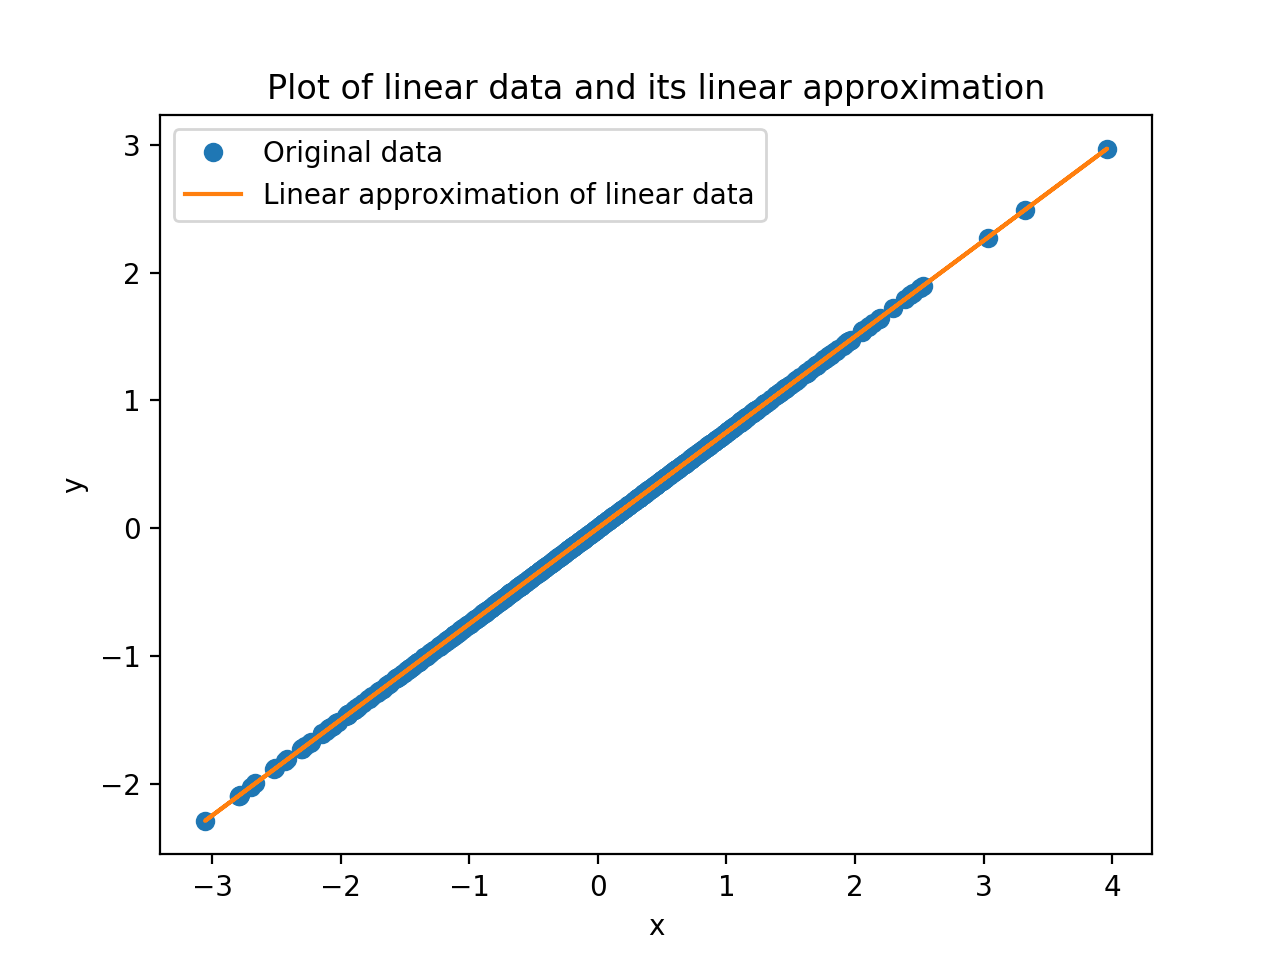
\includegraphics[width=0.7\textwidth]{../plots/task1_part1.png}
\caption{Plot of the linear data and its linear approximation}
\label{fig:task1_1}
\end{figure}
Part 2: \\
In the second part we use a nonlinear dataset from the "nonlinear\_function.txt" file and tried to approximate the function in a linear way again.
Figure \ref{fig:task1_2} shows then original data in blue again. The linear approximation of the function is  shown in orange. It can be easily seen that the linear approximation fits very bad. The reason for that is that the function is nonlinear and we try to approximate it linearly.
\begin{figure}[H]
\centering
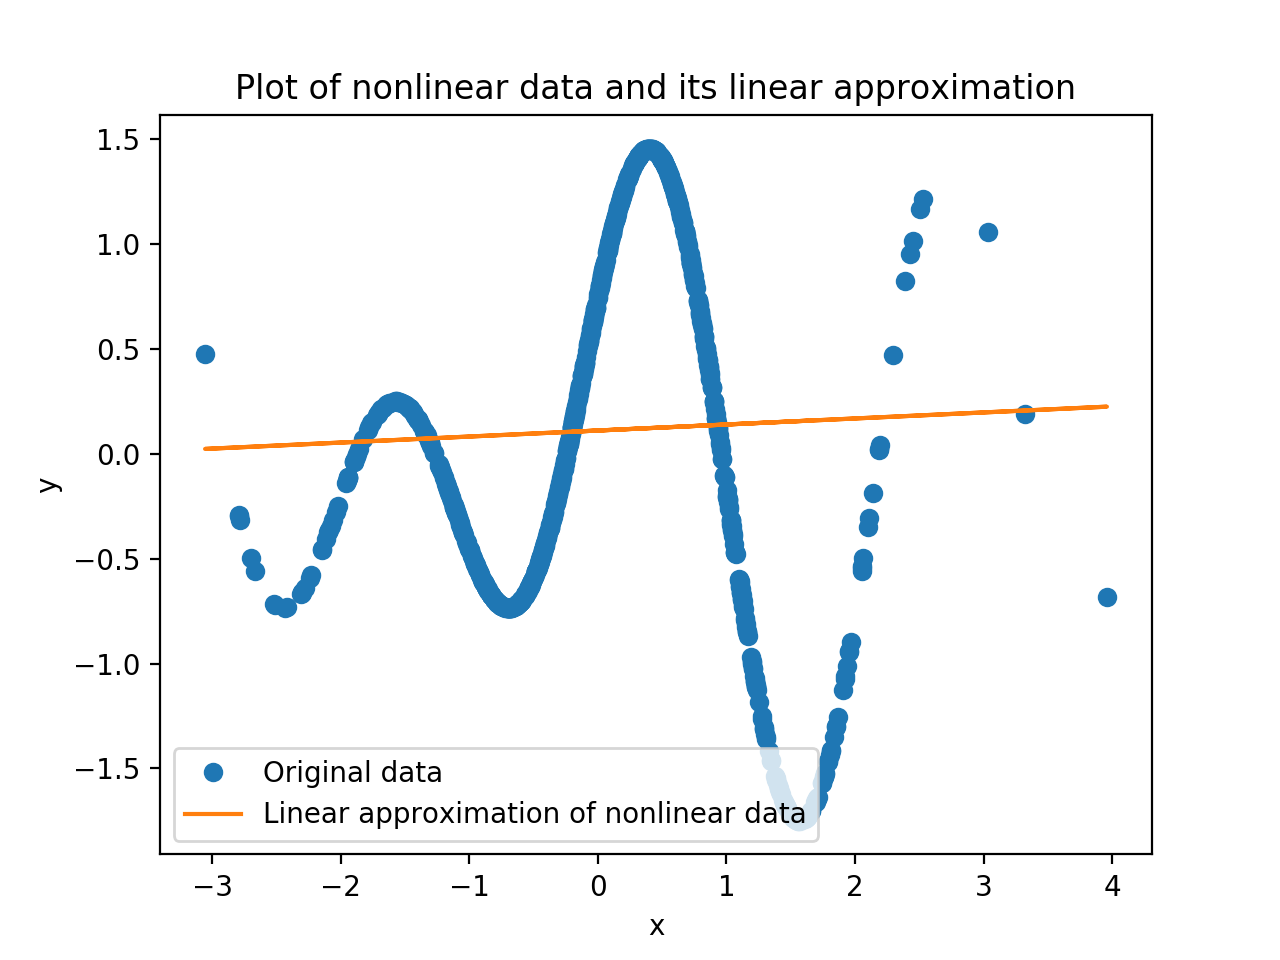
\includegraphics[width=0.7\textwidth]{../plots/task1_part2.png}
\caption{Nonlinear data and its linear approximation}
\label{fig:task1_2}
\end{figure}
Part 3: \\
After we tried to approximate the nonlinear dataset with a linear function in part 2, we now try to approximate the unknown nonlinear function f with a combination of radial basis function:
\begin{equation*}
	f(x)=\sum_{l=1}^Lc_l\phi_l(x), c_l \in \mathbb{R}^d
\end{equation*}
A radial basis function $\phi$ is defined as follows:
\begin{equation*}
	\phi_l(x) = \exp(-||x_l -x||^2/\epsilon^2)
\end{equation*}
where $x_l$ is the center of the basis function and usually just a random point of the data set. There is one $x_l$ for each radial basis function. \\
The minimal least square error problem looks similar to the linear case:
\begin{equation*}
\min_{\hat{f}} e(\hat{f}) =  \min_{\hat{f}} ||F-\hat{f}(X)||^2  =\min_C||F-\phi(X)C^T||^2
\end{equation*}
Here the matrix C contains as the matrix A for the linear case the coefficients $c_l$ and 
\begin{equation*}
\phi(X):= (\phi_1(X),\phi_2(X), \dots, \phi_L(X))
\end{equation*}
\\ We have to choose how many basis functions L  we use to approximate the nonlinear function. Besides, we have to choose $\epsilon$ appropriately.
Figure \ref{fig:task1_3} shows the original data in blue and the approximated function which makes use of radial basis functions in orange. It can be easily seen that the approximation is by far better than the linear approximation of part 2. \\ In general the approximation fits the original function quite well.
We chose $\epsilon$ according to the $\epsilon$ in the diffusion maps task of the previous exercise sheet. This means we computed the distance matrix among all the x values and took the maximum value for $\epsilon$. This meaximum value is multiplied by 0.05. Besides, we use $L=15$ radial basis functions for the nonlinear approximation.
\begin{figure}[H]
\centering
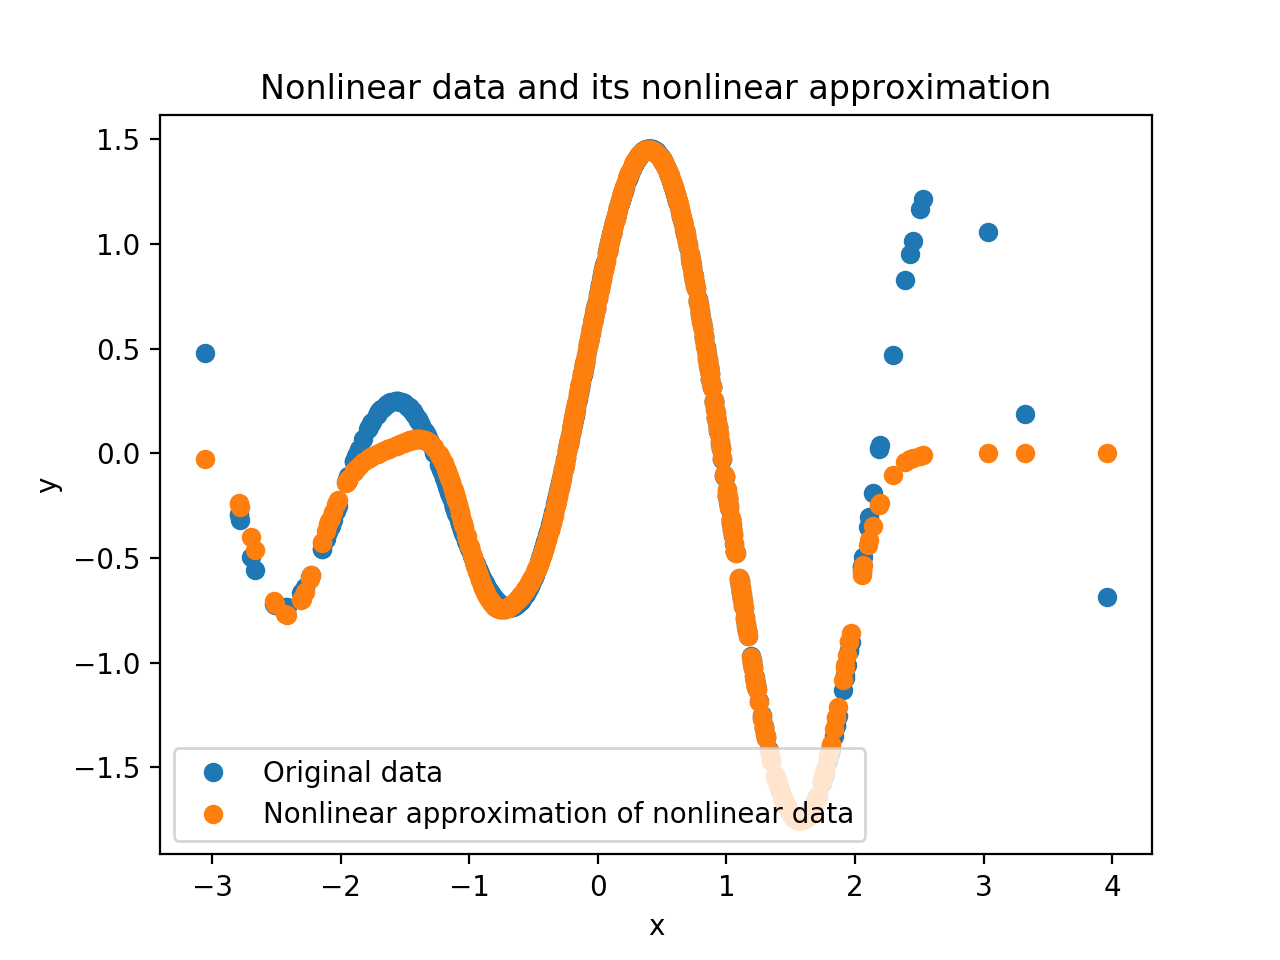
\includegraphics[width=0.7\textwidth]{../plots/task1_part3_eps.png}
\caption{Nonlinear data and its nonlinear approximation with radial basis functions}
\label{fig:task1_3}
\end{figure}
It is not a good idea to use radial basis functions to approximate a linear function such as the linear data set of A. You can use the radial basis functions to approximate a linear data set, but you should use a linear approximator, because the computational cost of the radial basis function is higher due to the fact that the distance matrix for all x has to be computed to determinate $\epsilon$. Besides the parameters of L and $\epsilon$ have to be chosen appropiately to obtain a good approximation.
\end{task}

\begin{task}{2, First step of a single pedestrian}
Part 1: \\
We use the pandas read\_csv function to read the text files containing two dimensional x0 and x1 data. We estimate the vector fields $v^{(k)}$ for each x0, using the finite-difference formula, given hereby:
\begin{equation*}
\hat{v}^{(k)} = \frac{x_1^{(k)} - x_0^{(k)}}{\Delta t}
\end{equation*}
Then we approximate the matrix $A$ such that:
\begin{equation*}
v(x_0^{(k)}) = v^{(k)} = Ax_0^{(k)}
\end{equation*}
An interesting thing to note is that, bias b is not added in this equation. This will have implications to the prediction later on. It will be mentioned in part 3.

For this purpose, we use the linear approximator implementation from task 1. As mentioned before the goal is to estimate the matrix $A$, such that the mean square error is minimized. This can be represented through the following equation:
\begin{equation*}
\min_{\hat{f}}e(\hat{f}) = \min_{\hat{f}}||F-\hat{f}(X)||^2 = \min_{A}||F-XA^T||^2
\end{equation*} \\

Part 2: \\
After fitting the linear approximator, we predict the vector fields, $\hat{v}^{(k)}$ for each x0. Then we use $\hat{v}^{(k)}$ with $\Delta t = 0.1$ to calculate $\hat{x1}^{(k)}$ using the formula.
\begin{equation*}
\hat{x1}^{(k)} = \hat{v}^{(k)}\Delta t + x0^{(k)}
\end{equation*}
We compare $x1^{(k)}$ and $\hat{x1}^{(k)}$ using the mean squared error formula and obtain the value of: 1.0532185339804091e-13 \\\\
Part 3: \\
We set $x0=(10, 10)^{(0)}$ and then estimate $\hat{v}^{(0)}$. We calculate $\hat{x1}^{(0)}$ using the equation given in part 2. Then using the corresponding $\hat{x1}^{(k-1)}$, we calculate the vector field $\hat{v}^{(k)}$ for it. We repeat this process for $T = 100$. We use steps of $\Delta t = 0.1$, so the total number of iterations are $\frac{T}{\Delta t} = 1000$. 
As seen in the figure \ref{fig:task2_3}, the motion stops at (0,0). We think that reason for this is that, we do not add bias term b to the linear approximator equation. Hence when $x=0$, then the matrix A has no effect on $\hat{x}$.

\begin{figure}[H]
\centering
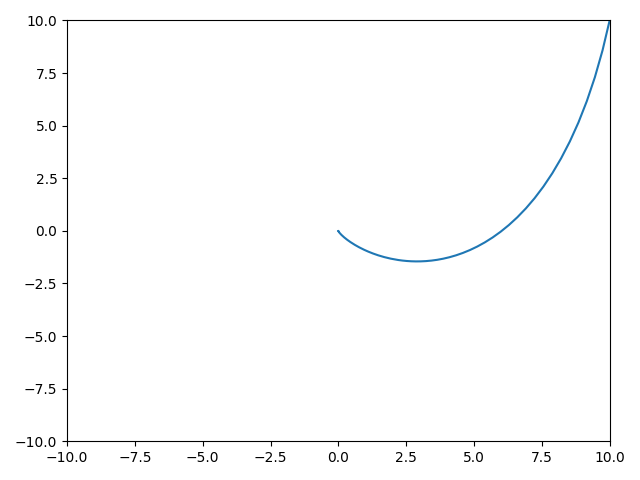
\includegraphics[width=0.6\textwidth]{../plots/task2_part3.png}
\caption{Trajectory of the motion}
\label{fig:task2_3}
\end{figure}

The phase portrait is given hereby:
\begin{figure}[H]
\centering
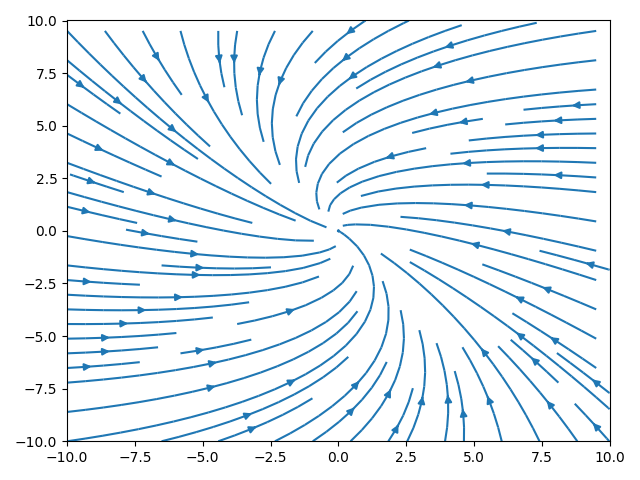
\includegraphics[width=0.6\textwidth]{../plots/task2_part3_phase.png}
\caption{The phase portrait}
\label{fig:task2_3_phase}
\end{figure}

\end{task}

\begin{task}{3, Approximating nonlinear vector fields}
Part 1: \\
At first we approximate the vector field $\hat{v}^{(k)}$ for every intial point $x_0^{(k)}$ with the equation:
\begin{equation*}
\hat{v}^{(k)} = \frac{x_1^{(k)} -x_0^{(k)}}{\Delta t}
\end{equation*}
Afterwards we try to estimate the vector field describing $\psi$ with a linear operator $A \in \mathbb{R}^{2\times2}$ such that
\begin{equation*}
\frac{\partial}{\partial t} \psi(t,x) \approx \hat{f}_{linear}(x) = Ax
\end{equation*}
After getting A we approximate $\hat{x}_1^{(k)}$ and compute the mean squarred error between the approximated and the known end points for a chosen $\Delta t = 0.5$.
The mean squared  error is defined as follows:
\begin{equation*}
\sum_{k=1}^N ||\hat{x}_1^{(k)} - x_{1}^{(k)}||^2
\end{equation*}
The mean squared error is 75.54.\bigbreak
Part 2: \\
Part 2 is similar to part 1, but this time we approximate the vector field using radial basis functions such that
\begin{equation*}
\frac{\partial}{\partial t}\psi(t,x) \approx \hat{f}_{rbf}(x) = C \phi(X)
\end{equation*}
 We choose $L=10$ and take  for $\epsilon$ the biggest value of a distance matrix between all initial points $x_0$.
The mean squared error is 0.24. \\
The mean squarred error is extremely low, so the performance of the nonlinear approximator is very good. Consequently you can see that the vector field is nonlinear. Otherwise the mean squared error of the linear approximation would be lower.
You can see that the difference between both mean squared errors is high, because the mean squared error of the nonlinear approximated vector field is very low. \bigbreak
Part 3: \\
For this part we use the nonlinear approximator, because in our opinion the vector field is nonlinear and therefore the nonlinear approximator shows better performance in comparison to the lineaer approximator. We use the approximated vector field to solve  the system for a larger time with all intitial points $x_0$.\\
Figure \ref{fig:task3_part3} shows the trajectories for the system at the end state. You can see several steady states. The steady states are at the following coordinates: \bigbreak
\begin{tabular}{|l|c|c|c|c|}
\hline
x-coordinate of steady state& -2.92&3.22&3.65&-4.26\\
y- coordinate of steady state& 3.13&1.85&-1.27&-3.65\\
\hline
\end{tabular}
\begin{figure}[H]
\centering
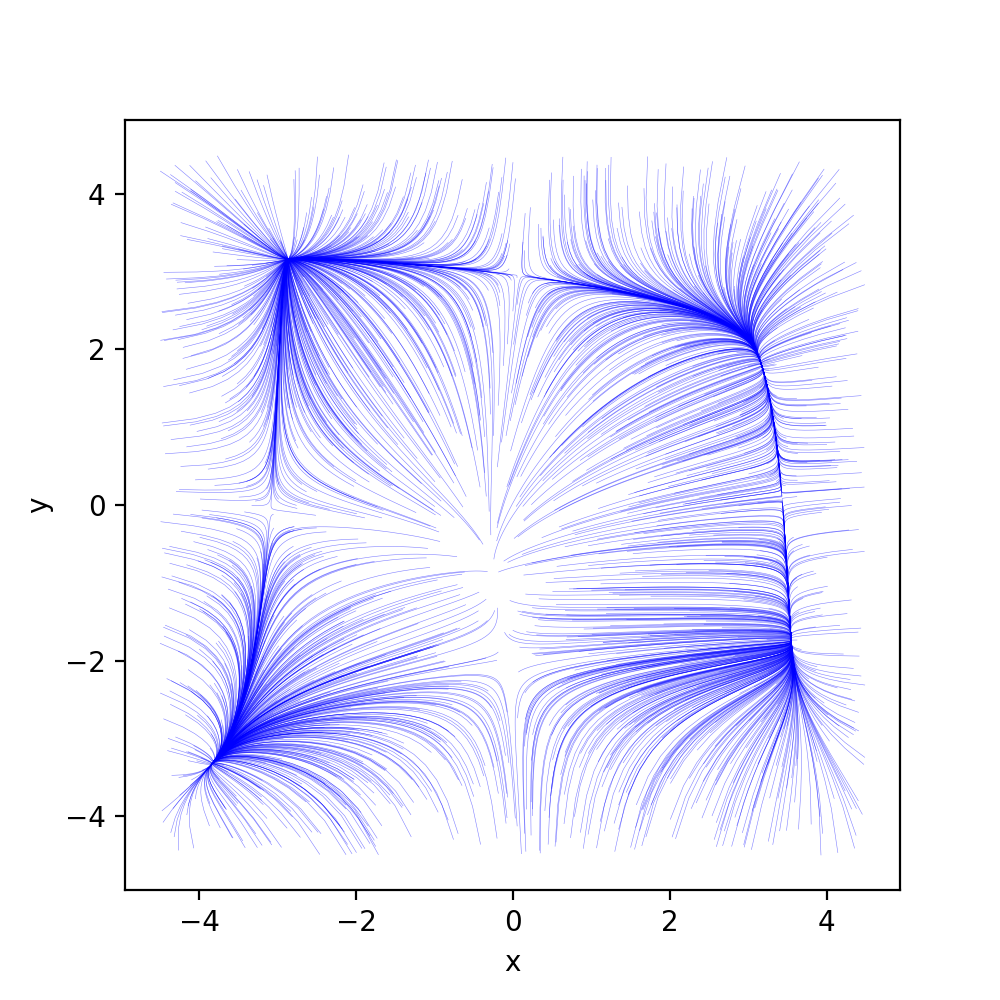
\includegraphics[width=0.7\textwidth]{../plots/task3_part32.png}
\caption{Trajectories of the system at the end state starting at the intial points $x_0$}
\label{fig:task3_part3}
\end{figure}
The system can be topologically equivalent to a linear system.
\end{task}

\begin{task}{4, Obstacle avoidance}
Part 1: \\
We read the takens.txt file using the read\_csv function from pandas library. We plot the first coordinate (column) of the data against time t. \ref{fig:task4_part1_1}

\begin{figure}[H]
\centering
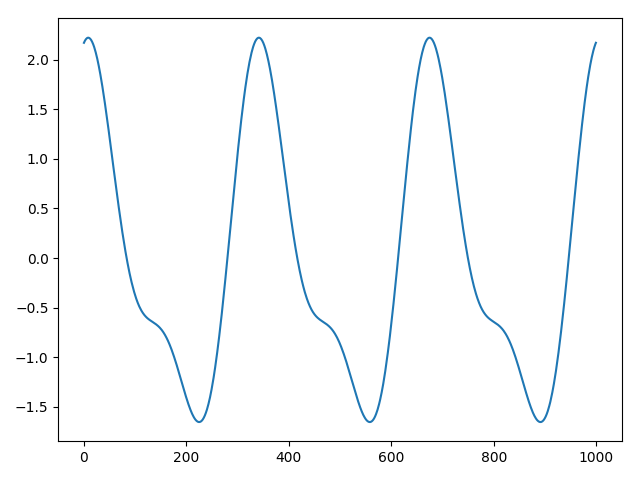
\includegraphics[width=0.6\textwidth]{../plots/task4_part1_1.png}
\caption{The plot of first coordinate against time t}
\label{fig:task4_part1_1}
\end{figure}

Then we plot a time delayed version of the first coordinate against itself. The first coordinate is delayed by $\Delta n = 70$, because we observe the first plot and measure the time it takes for the first coordinate to complete a fourth of the periodic cycle. \ref{fig:task4_part1_2}

\begin{figure}[H]
\centering
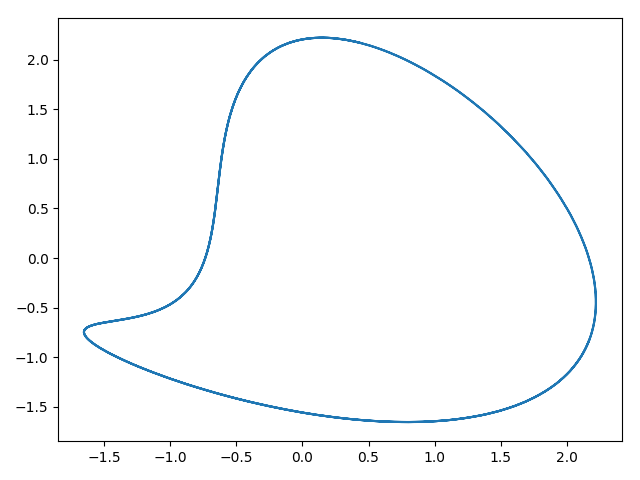
\includegraphics[width=0.6\textwidth]{../plots/task4_part1_2.png}
\caption{The plot of the first coordinate against the time delayed version of the first coordinate}
\label{fig:task4_part1_2}
\end{figure}

We know that Takens has shown that embeddings with $d^{e} > 2n$ will be faithful generically so that there is a smooth map:
\begin{equation*}
f : \mathbb{R}^{d^{e}} \rightarrow \mathbb{R}
\end{equation*}

where $d^{e}$ is the embedding coordinates and n is the number of coordinates of the data. Hence, as the data has two coordinates, so according to Takens, atleast 5 time delayed embedding coordinates will be needed to make sure that the periodic manifold is embedded correctly. \\\\

Part 2: \\
We use the lorenz attractor implementation from Exercise 3 in this part. Using the solve\_ivp function from the Sklearn library we calculate the x, y and z coordinates of the trajectory, after setting the initial position as (10, 10, 10). \ref{fig:task4_part2_1}

\begin{figure}[H]
\centering
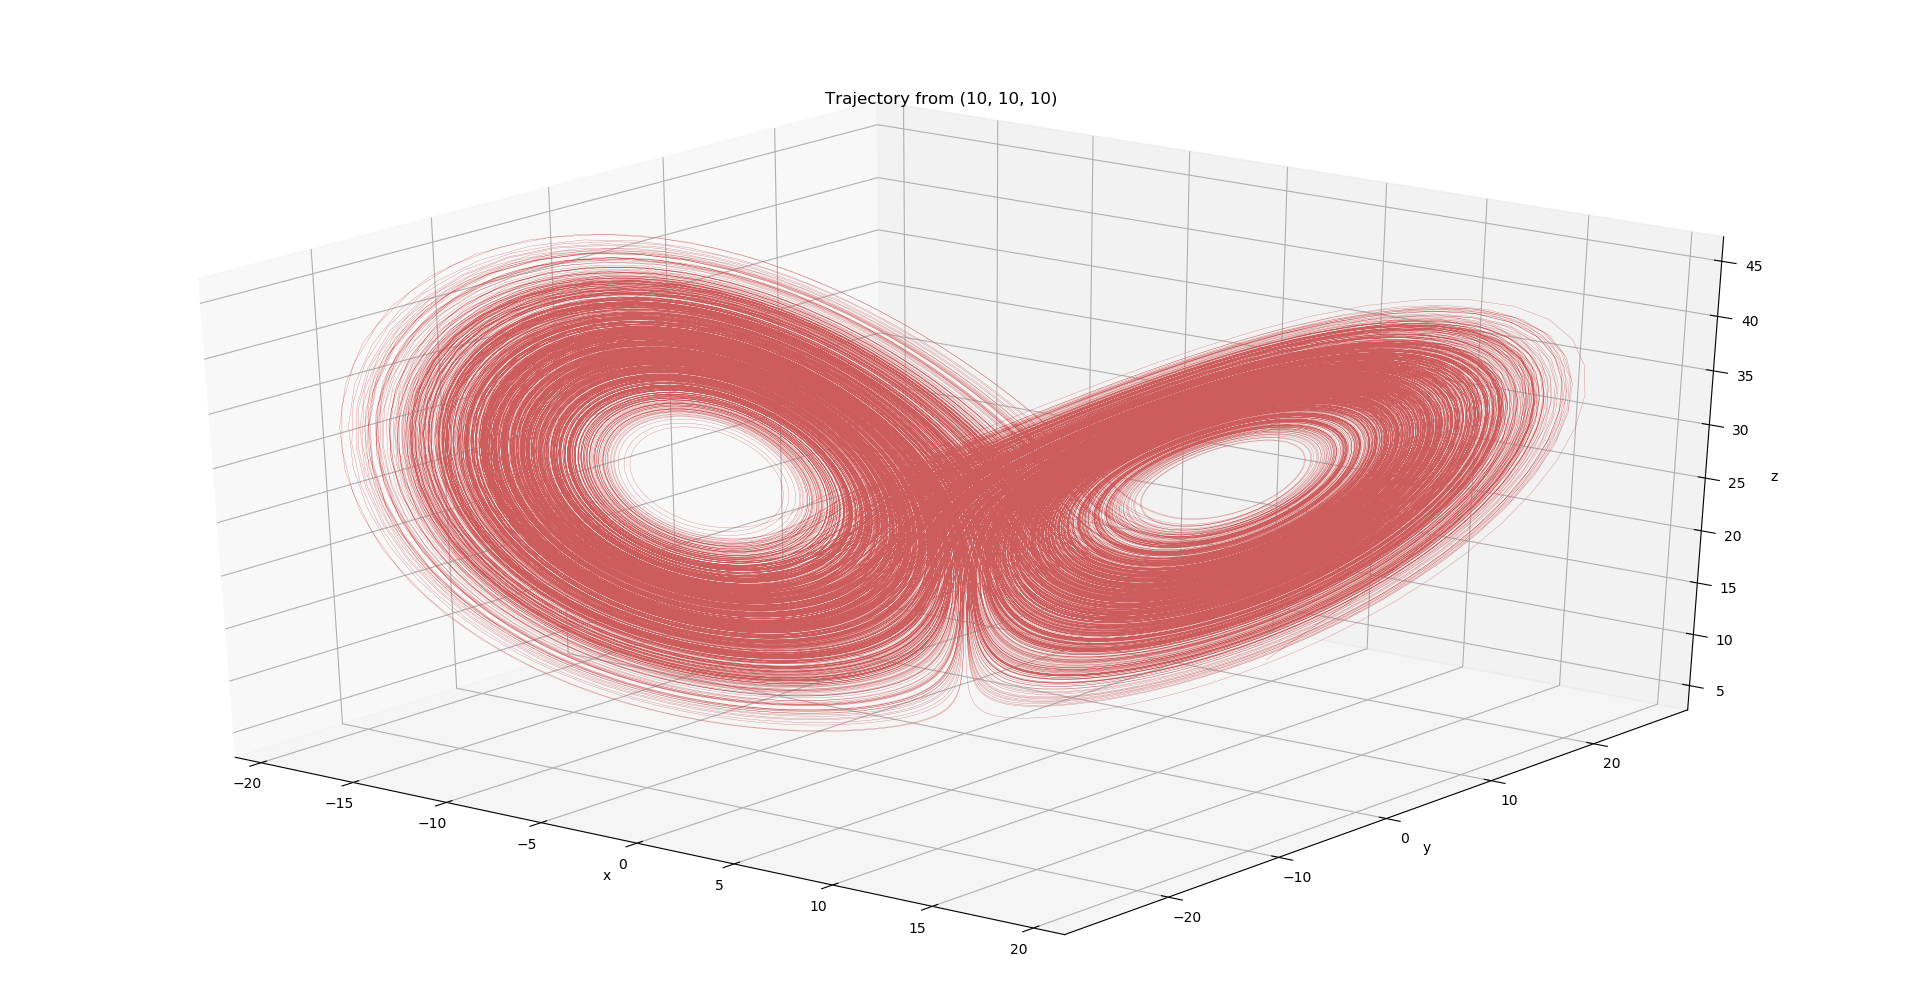
\includegraphics[width=0.7\textwidth]{../plots/task4_part2_1.png}
\caption{Plot of the lorenz attractor trajectory}
\label{fig:task4_part2_1}
\end{figure}

Then we obtain the x-coordinate as $x0 = x(t)$ then we plot x0 against $x1 = x(t + \Delta t)$ and $x2 = x(t + 2\Delta t)$. We set $\Delta t = 18$. \ref{fig:task4_part1_2}

\begin{figure}[H]
\centering
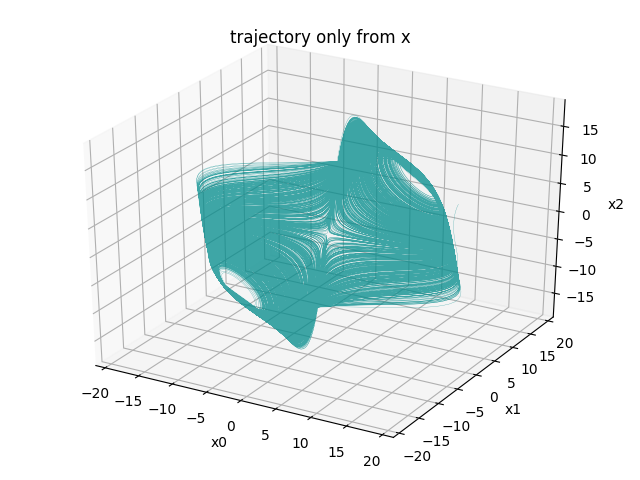
\includegraphics[width=0.6\textwidth]{../plots/task4_part2_2.png}
\caption{Plot of x0, x1 and x2 in a 3 dimensional space}
\label{fig:task4_part2_2}
\end{figure}

Lastly, we obtain the z-coordinate from the solve\_ivp result that we obtained earlier, as $z0 = z(t)$ then we plot z0 against $z1 = z(t + \Delta t)$ and $z2 = z(t + 2\Delta t)$. We set $\Delta t = 20$. \ref{fig:task4_part2_3}

\begin{figure}[H]
\centering
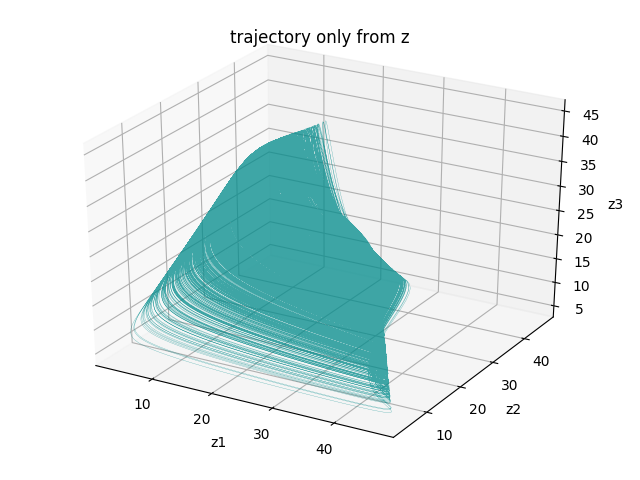
\includegraphics[width=0.6\textwidth]{../plots/task4_part2_3.png}
\caption{Plot of z0, z1 and z2 in a 3 dimensional space}
\label{fig:task4_part2_3}
\end{figure}

Plotting z0, z1 and z2 does not result in a representative visualization of the original data, compared to the plot of x0, x1 and x2. The reason for this is that, lorenz attractor system consists of three ordinary differential equations. The differential equation responsible for the z-coordinate has the z-coordinate term in it but when using time delayed embedding, the subsequent time delayed coordinates z1 and z2 do not account for this. It results in the error propagating through the embedding. \\\\

Part 2, Bonus task: \\
Using the x0, x1 and x2 coordinates obtained in the previous task, we approximate the vector fields $v^{(k)}$ at each timestep using the finite-difference formula. Then we fit the non-linear approximator to predict the $\hat{v}^{(k)}$ given the embedding coordinates.

The next step is to use the fitted linear approximator as the vector field predictor and using the solve\_ivp function from Sklearn library to generate the trajectories. The starting point is set as the first point of the embedding coordinates. The results obtained are not good. Even though the resulting trajectory loops, it does not resemble the trajectory of the training data.

\begin{figure}[H]
\centering
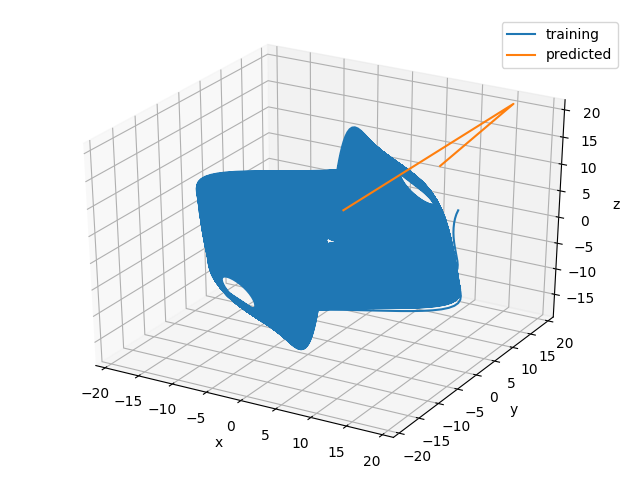
\includegraphics[width=0.6\textwidth]{../plots/task4_part2_bonus.png}
\caption{Comparison of the training and predicted data}
\label{fig:task4_part2_bonus}
\end{figure}

Part 3: \\
We used the old implementation of pedestrian trajectory parser from exercise 3 to get the coordinates of pedestrians in the case when the path is not blocked by the object. As mentioned in the exercise we concatenate 200 time delay embedding into one data point and then using $\Delta t = 1$, we generate several data points. We obtain, 3551 data points from this process as the total number of data points in the original data was 3751. 
We use the PCA implementation from exercise 4 to obtain the first two principal components of the resulting data. \ref{fig:task4_part3}

\begin{figure}[H]
\centering
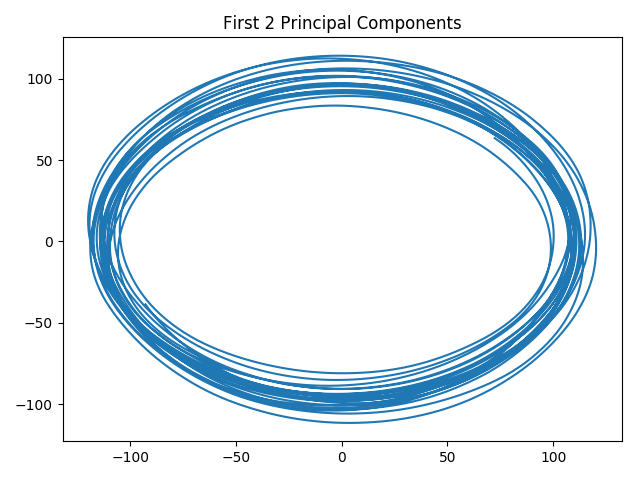
\includegraphics[width=0.6\textwidth]{../plots/task4_part3.png}
\caption{Plotting the first two principal components}
\label{fig:task4_part3}
\end{figure}

\begin{itemize}
 \item 
 \item as mentioned in the exercise
\end{itemize}
\end{task}

\begin{task}{5, Tests}
\begin{enumerate}
\item[TEST1:] RiMEA scenario 1 (straight line, ignore premovement time)\\
- not done, but citing RiMEA guidelines -
\item[TEST2:] RiMEA scenario 4 (fundamental diagram, be careful with periodic boundary conditions).\\
- test successful - 
\item[TEST3:] RiMEA scenario 6 (movement around a corner).\\
- test successful - 
\item[TEST4:] RiMEA scenario\\
- test successful - 
\end{enumerate}
\end{task}



\end{document}